%This file will be included in the ThesisMain Document as the experimentation
%section.

%Author: James Kelly
%Last Modified: 10-08-08

\begin{center}
\section{EXPERIMENTATION}
\end{center}

\subsection{Stormwater Discharge Simulations}

\subsubsection{Aggregate Samples}
An experiment was devised to measure a thermal exchange between water and a sample of gravel. To measure the exchange in a hydro-dynamic scenario, a so-called stormwater discharge simulator was constructed to flush a body of gravel with heated water at high rates for up to 5 minutes. Temperature sensors measured water temperature and provided time-based temperature data for an analysis of the heat exchange between water and aggregate. In each group of experimental trials, a family of 9 gravel or rock samples was measured (Table \ref{aggsam}), each with a packed volume of 5.60 liters (Appendix A). 

\begin{table}[t!]

\centering                           
\caption[Aggregate Samples]{\textbf{Aggregate Samples}\label{aggsam}} 
\begin{tabular}{l c c c c c c}              
\hline\hline
\\                               
 Material & Diameter & Mass (kg) & ISS (L) & $\frac{n}{kg}$ & Bulk $\rho\;\frac{kg}{L}$
\\[1ex]
\hline 
\\
% Entering 1st row
& $\frac{3}{8}$'' 	& 8.70 	& 2.367	& 1123 	& 1.56\\[1ex]
& $\frac{1}{2}$'' 	& 6.90 	& 2.598	& 201 	& 1.24\\[1ex]
\raisebox{0 ex}{Quartzite}
& $\frac{3}{4}$'' 	& 7.05 	& 2.786	& 80 	& 1.27\\[1ex]
& 5'' 			& 9.00 	& 3.088	& 3 	& 1.62\\[1ex]
\\
\hline
\\
& $\frac{5}{8}$'' 	& 6.35 	& 3.480 & 196 	& 1.14\\[-1ex]
\raisebox{2ex}{Crushed Brick}
& 1'' 			& 5.90 	& 3.556	& 57 	& 1.06\\[1ex]
\\
\hline
\\
& $\frac{5}{8}$'' 	& 7.50 	& 2.608	& 184 	& 1.35\\[-1ex]
\raisebox{2ex}{Marble Cobbles}
& 1'' 			& 7.05 	& 2.675	& 47 	& 1.27\\[1ex]
\\
\hline
\\
Stream Cobble 		& 2'' 	& 10.4 	& 2.556	& 20 & 1.87\\[2ex]
\\
\hline
\\
Siltstone 		& $\frac{1}{2}$'' & 8.9 & 3.191 & 7 & 1.60\\[1ex]
\\
\hline
\\
Steel Balls (1018)	& 1'' 	& 25.0 	& 3.29 	& 15 & 4.50\\[1ex]
\\
\hline
\\
Glass Marbles		& 1''	& 6.50	& 3.21	& 52 & 1.17\\[1ex]
\\
\hline\hline
\end{tabular}
\label{tab:AggSam}
\end{table}

Quartzite and metasiltstone gravel samples were acquired from a local quarry that processes only construction aggregates that are mined on site. These samples include a range of sizes crushed for general construction and asphalt production. Quartzite aggregates are noted for their irregular cobble geometry and relatively high Mohs hardness of 7, which makes it especially suitable for use in non-partitioned arrangements \citep{ballast}. The other samples were acquired from a local landscaping retailer. Marble garden rocks, though comparably exotic, were selected for their especially high density and heat capacity. The brick sample was simply red, crushed construction brick that was sorted into two general sizes. Round river cobble and red colored medium siltstone were selected for shape and material variation. Finally unplated, mild steel balls (1018 non-annealed alloy) and glass marbles were also tested primarily as theoretically ideal aggregates in one or more thermal parameters.

\subsubsection{Temperature Measurement}
In measuring temperature, HOBO sensors by Onset Solutions were launched and used for each trial, with data being collected from each sensor after every experiment. Each sensor was ultimately modified to provide a 3 second temperature responsivity, as default manufacturer times are well over 5 minutes. The modification involved moving the temperature themistor to the outside of the sensor casing so that it was directly in contact with the fluid, and then re-sealing the unit. 

In Figure (\ref{modSens}) the sensor modification is visible as the protruding temperature element from the end of the sensor body. The semi-conductor that generates the signal for the sensor circuit is encased in a small, black epoxy bulb and this was filed down to further decrease the thermal responsivity with some success. The hole that was drilled in the plastic sensor case was sealed with a a hot/cold temperature cyanoacrylate cement. Before final reassembly, the sensor cavity was filled with a household expanding foam to further protect the sensor circuit from water infiltration. A typical failure mode for this modification was the sensor wires cracking and consequently causing a short circuit. 

\begin{center}
\begin{figure} [h!]
 \centering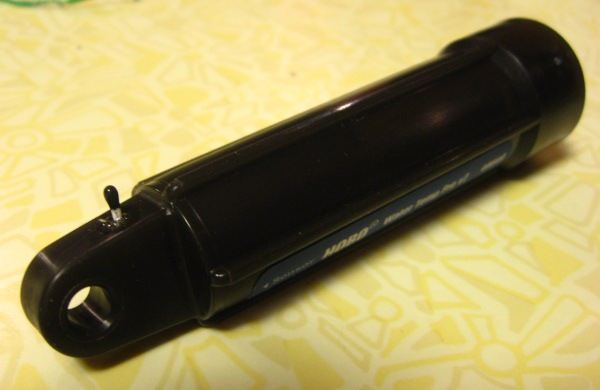
\includegraphics[scale=0.8]{modSensor.jpg}
 \caption[Modified HOBO Sensor]{\textbf{\emph{A modified HOBO sensor}} This shows a HOBO temperature sensor modified to provide better thermal responsivity.\label{modSens}}
\end{figure}
\end{center}

Sensors used in all trials were first matched and calibrated by immersing them in heated fluids and selecting the sensors that only had similar readouts for responsivity and temperature. The modifications induced a greater variance on sensor accuracy, and so this process was implemented to control that. The sensor sampling rate was 1 second, and it was found that the sensors acheived about 50\% true value within that time frame under the most extreme temperature differences. Under the temperature differences found in a single trial, it was observed that such true temperature readings within a sample cycle were much closer, within a degree. 

Measurement error in all data originates with the sensors. There is a temporal error associated not only with just the thermal responsivity but additionally with the synchronization of individual sensors with respect to one another. This synchronization error was found to be up to 1 second in difference and is sourced to the software and personal computer when the sensors are launched. Top and bottom sensors were always carefully ``matched'', in that they measured temperatures very near one another with nearly the same responsivity. A true temperature is not as critical since all fundamental results were interpreted from a temperature difference.

\begin{center}
\begin{figure}[h!]
 \vspace{25mm}
 \centering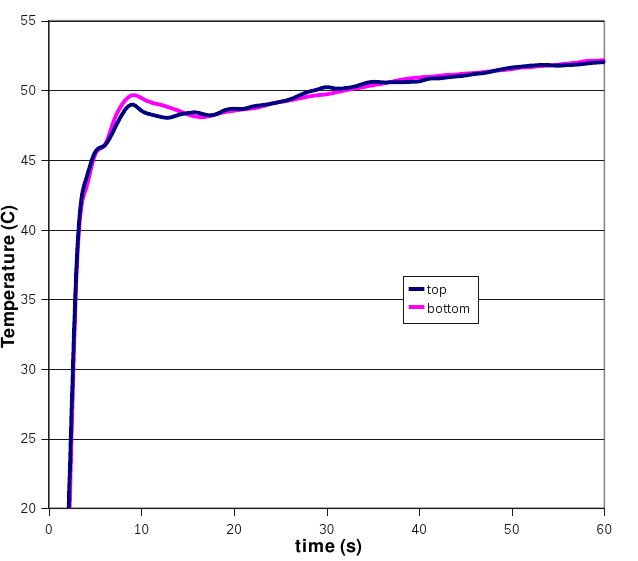
\includegraphics[scale=0.6]{sensorComp1.jpg}
 \caption[Sensor Responsivity]{\textbf{\emph{A comparison of a modifed top and bottom HOBO sensor}} Sensors that had similarly fast responsivity after modification were used to measured the temperature differences across the sample vessel. This match was performed for each trial.\label{sensComp}}
\end{figure}
\end{center}

\begin{landscape}
\begin{center}
\begin{figure}
 \centering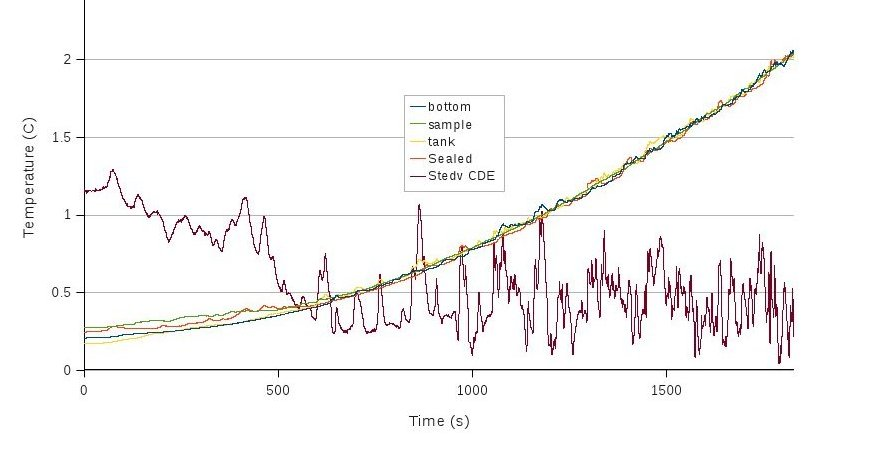
\includegraphics[scale=0.6]{sensorComp2.jpg}
 \caption[Sensor Comparison]{\textbf{\emph{A comparison of modified sensors over a wide temperature range}} This test was performed after a modifcation was implemented to test the long term temperature stability and reliability of modified sensors. In this test, the sensors were immersed in a cold water bath that was slowly heated.\label{sensComp2}}
\end{figure}
\end{center}
\end{landscape}

\subsubsection{Apparatus Construction Basics}
An apparatus was constructed to measure the ability of an aggregate sample to thermally sink a continuous flow of heated water. The apparatus consisted of a main circuit through which heated water was continuously circulated from a reservoir and afterwards discharged. The vessel that contained the aggregate sample was oriented vertically, with hot water introduced at the top of the vessel. Using HOBO sensors, flow temperature was measured before the water entered the sample vessel, and after. A flow sensor measured the flow rate shortly after the sample vessel. Figure (\ref{discharger}) is a schematic illustration of the apparatus, its flow design and the sensor loctions. Photographs of the operational apparatus are shown in Figures (\ref{dischargerPhoto}) and (\ref{vesselPhoto}). 

\begin{center}
\begin{figure}
\noindent
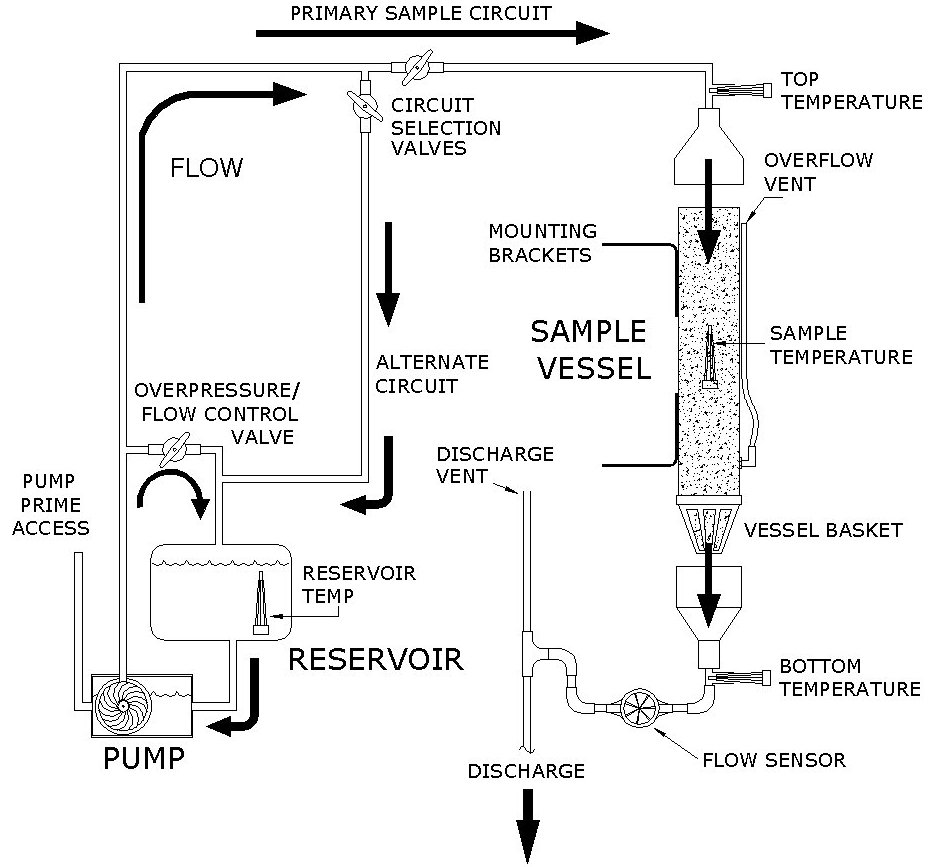
\includegraphics[scale=0.5]{DISCHARGER.jpg}
\caption[Stormwater Discharge Simulator Schematic]{\textbf{\emph{Schematic Diagram of the Stormwater Discharge Simulator}}\label{discharger}}
\end{figure}

\begin{figure}
 \centering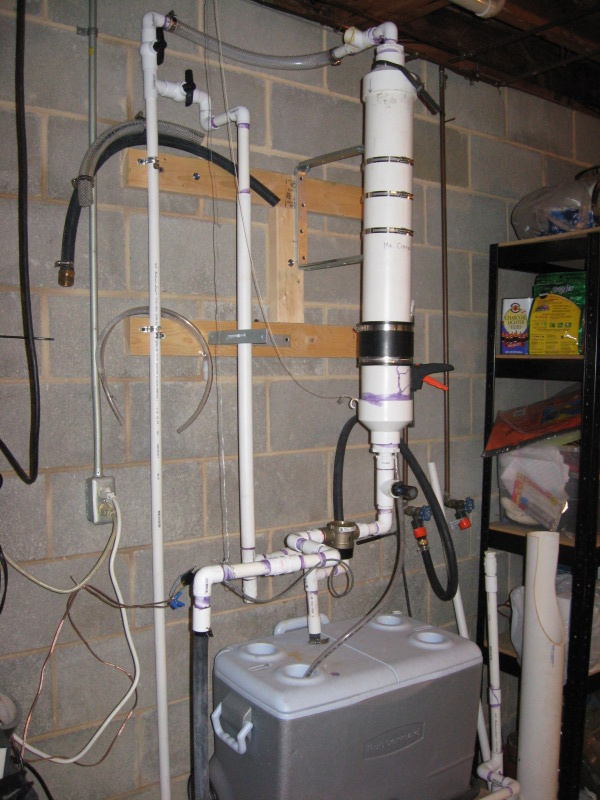
\includegraphics[scale=1.25]{dischargerPhoto.jpg}
 \caption[Stormwater Discharge Simulator]{\textbf{\emph{The assembled stormwater discharge simulation apparatus.}}\label{dischargerPhoto}}
\end{figure}
\end{center}

\begin{figure}
\centering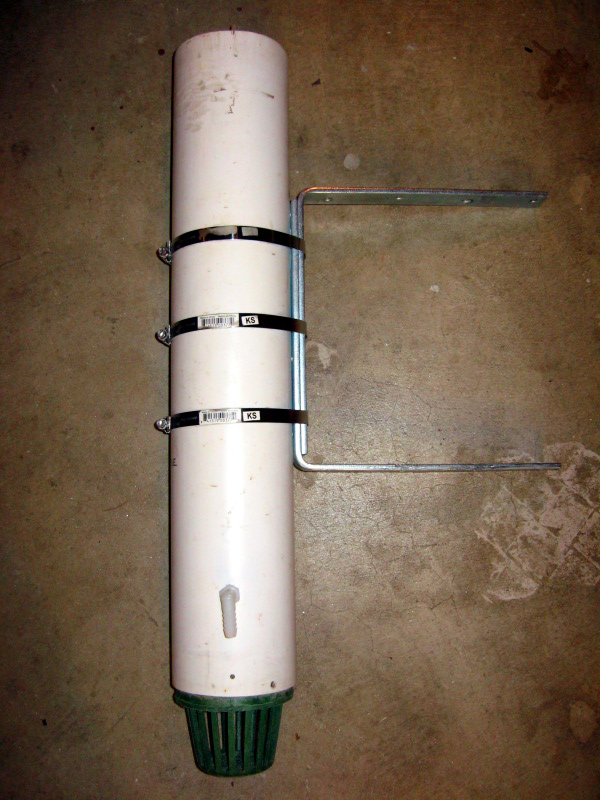
\includegraphics[scale=1.25]{vesselPhoto.jpg}
\caption[Sample Vessel]{\textbf{\emph{Sample vessel is shown seperated from the main circuit.}}\label{vesselPhoto}}
\end{figure}

\subsubsection{Apparatus Operation}
A sample or aggregate material was dumped into the vessel, which was removed from the main circuit. Figure (\ref{isovessel}) illustrates a cross section of the sample vessel, the sample aggregate and the vessel dimensions. The sample was checked for correct packing and the vessel was installed into the main circuit to complete the assembly of the apparatus. The reservoir was filled with 40 liters of water typically heated to 45-50 $^{o}$C. Run-time specifics are tabulated in Table (\ref{runTime}).

\begin{figure}[h!]
\centering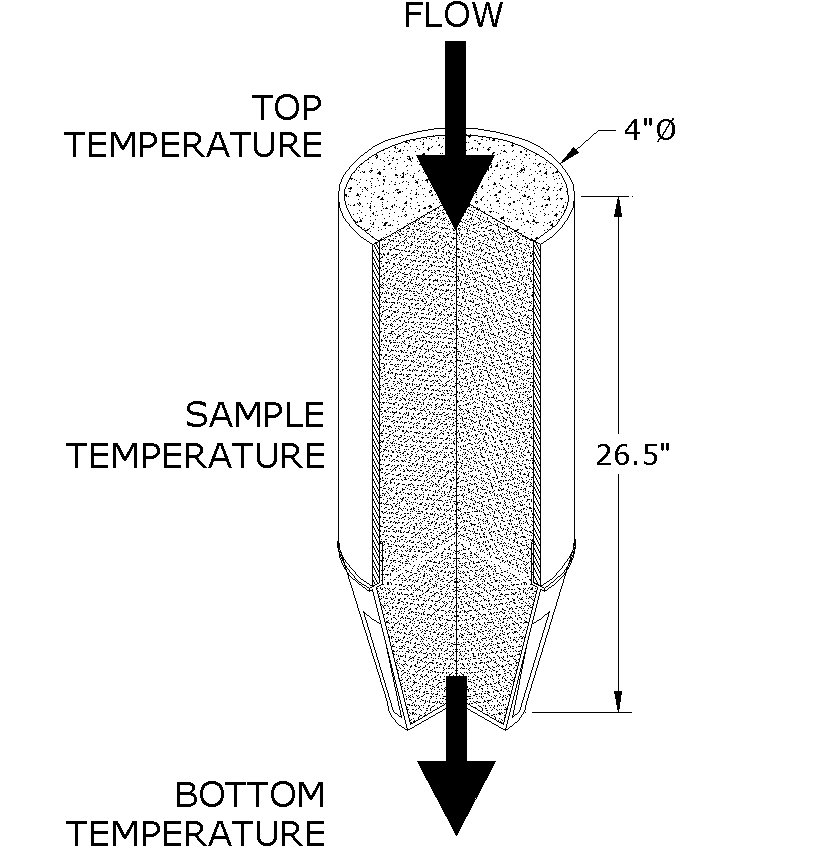
\includegraphics[scale=.35]{isoVessel.jpg}
\caption[Sample Vessel Cross Section]{\textbf{\emph{Sample vessel dimensions and cutaway with temperature probe locations.}} (The figure is not drawn to scale.)\label{isovessel}}
\end{figure}

An electric centrifigal pump was used to circulate water from the reservoir up to the top of the sample vessel. The pumping rate was adjustable with a gate valve that returned a certain fraction of the flow to the pump prime. The sample vessel was 4'' in diameter and 26.5'' in length, cut from a length of schedule 40 PVC. A drainage basket was fitted into the end to restrain the sample, yet afford minimal flow obstruction. The vessel performed as a gravitationally charged fluid coupling, through which water freely flowed through the interstitial space of the aggregate. Because gravity drives the flow, the type of aggregate not the pumping rate, was the dominant control of flow in the vessel. It should be noted that the maximum flow rate produced by the pump was accomodated by all aggregate samples. This was verified by the use of a clear overflow vent tube installed in the side of the sample vessel. If the net inflow were to exceed the effluent, the accumulation of fluid relative to the vessel height would appear in the clear vent tube, and this was never observed during a trial in which data was collected.

A second flow circuit was used to circulate water before the trial was to begin. This second circuit paralleled the primary sample circuit, except branching off just prior to the top temperature sensor and bypassing the sample vessel, returning all water to the reservoir. This circuit was used for 2-3 minutes prior to flushing the sample, and then disabled with a gate valve once the main circuit was opened. This recirculatory circuit was used to flush out cold pump prime water and to heat the circuit piping and brass pump head prior to collecting data. This warm-up helped to normalize the energy flow into the sample vessel and provided an initial thermal charge with a temperature closer to the actual reservoir temperature. The reservoir temperature dropped nominally when turning on this circuit. 

\begin{table}[ht!]
\caption[Experiment Nomenclature]{\textbf{Experiment Nomenclature}\label{simNom}}
\centering
\begin{tabular}{r l l}
Parameter & Abbreviation & Units\\
\hline
\\[-.5ex]
Fluid (Water)					&	$W$\\[3mm]

Aggregate Material or Sample			& 	$R$\\[3mm]

Energy						&	$Q$			& $J$\\[3mm]

Net Energy Exchange [Source -- Sink]		&	$Q_{net}[W-R]$		& $J$\\[3mm]

Time Step Energy Exchange [Source -- Sink]	&	$Q(t)[W-R]$		& $J$\\[3mm]

Volumetric Heat Capacity of Fluid (Water)	&	$Cv_{W}$		& $\dfrac{J}{L*K}$\\[3mm]

Bulk Specific Heat of Aggregate			&	$c_{R}$			& $\dfrac{kJ}{kg*K}$\\[3mm]

Bulk Heat Capacity of Aggregate			&	$C_{R}$			& $\dfrac{kJ}{K}$\\[3mm]

Vessel Residency Time 				&	$t_{V}$			& $s$\\[3mm]

Aggregate Bulk Specific Gravity			&	$\rho_{R}$		&\\[3mm]

Aggregate Bulk Thermal Conductivity		&	$\kappa_{R}$		& $\dfrac{W}{m*K}$\\[3mm]

Aggregate Bulk Thermal Diffusivity		&	$\alpha_{R}$		& $\dfrac{m^{2}}{s}$\\[3mm]

Aggregate Mass					&	$m_{R}$			& kg\\[3mm]

Average Top Sensor Temperature 			&	$T[TOP]$		& $^{o}C$\\[3mm]

Time Stepped Bottom Sensor Temperature 		&	$T(t)[BOTTOM]$		& $^{o}C$\\[3mm]	

Fluid Flow Rate (L/s)				&	$\nu_{W}$		& $\dfrac{L}{s}$\\[3mm]

Top - Bottom Temperature Difference 		&	$\Delta T[TB]$		& $^{o}C$\\[3mm]

Time Stepped $\Delta T[TB]$ 			&	$\Delta T(t)[TB]$	& $^{o}C$\\[3mm]

Ambient Temperature				&	$T[AMBIENT]$		& $^{o}C$\\[3mm]

\hline
\end{tabular}
\end{table} 

\subsection{Flow Sensor Data Acquisition and Interface}
A rotary vane type flow sensor with a 3/4'' diameter aperature was placed inline with the outgoing flow. This particular sensor generated a digital 5V output signal that coincided with the flow rate. To generate this signal, the sensor itself was driven by 5V DC, rated at 40 mA. This digital signal was read by a single data input (address = 3F8h) on a personal computer parallel port. The port was sampled at 1kHz, which restricted the maximum measurable input signal to about 330 Hz. This was found to coincide with a flow rate of about 3 L/s, well below the apparatus' pump capacity.

On the personal computer, a data acquisition (DAQ) front panel (Figure \ref{frontpanel}) was coded in Visual Basic (6.0) to sample the parallel port and to convert the signal to a real-valued flow rate. The front panel was first calibrated using gravitationally driven flows of a known volume at various flow rates. An order 3 polynomial calibration curve was then formulated from this data and used by the front panel to determine flow rate. Errors encountered in the calibration of the flow sensor were two orders of magnitude less than the manufacturer's specificed measurement error of $\pm10\%$. 

\begin{figure}[ht!]
 \centering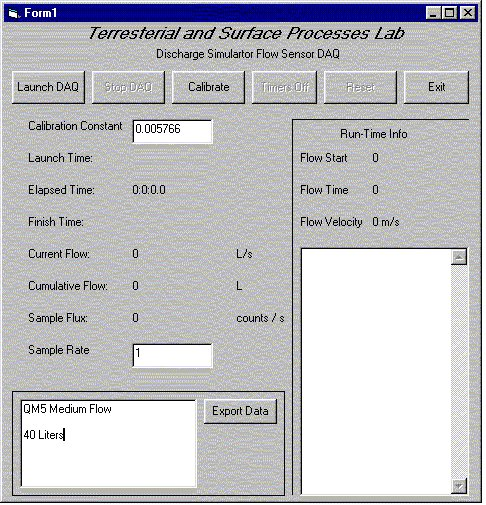
\includegraphics[scale=.65]{frontpanel.jpg}
 \caption[Front Panel Screen]{\textbf{\emph{Front Panel of the Data Acquisition (DAQ) interface}} This Visual Basic front panel was designed to time only active flow (non-zero) and to export the data batch as a tab-delimited ASCII text file. A high precision timer (RSTimer) was used to sample data from the parallel port at 1kHz, and to create flow rate data with one second resolution. Before each trial, this timer was synchronized with the temperature sensors.\label{frontpanel}}
\end{figure}

\begin{figure}[ht!]
 \centering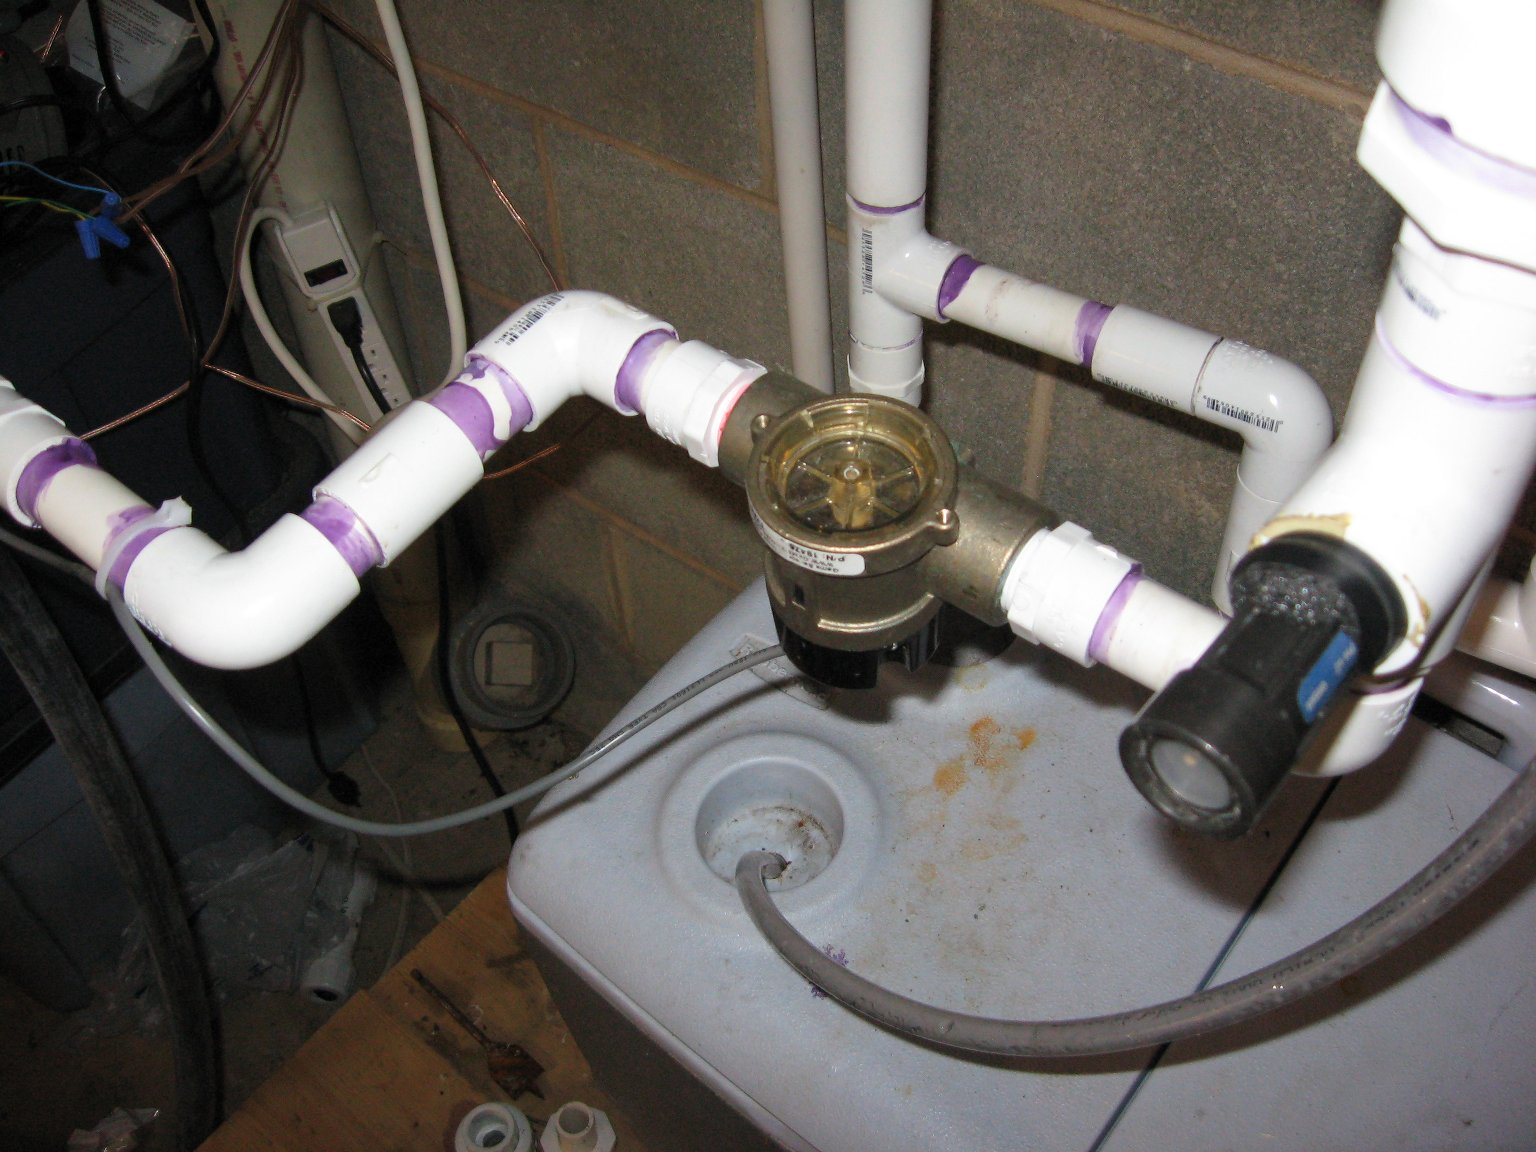
\includegraphics[scale=.25]{flowsens.jpg}
 \caption[Flow Sensor]{\textbf{\emph{Photograph of the Operational Flow Sensor}}\label{flowsenser} Shown is the rotary vane type flow sensor that was interfaced to the Visual Basic Front Panel. Visible is the bend in the plumbing following the sensor that served to create some backpressure to limit the air bubble ingestion of the rotary vane chamber.}
\end{figure}
\pagebreak
\subsubsection*{Run-Time Specifics}

When conducting a trial, the following procedure was followed to carry out a single flow experiment:

\begin{itemize}
 \item The two personal computers that manage data collection were time syncronized via a network connection. This was typically  done only once every hour. 
\pagebreak
 \item The temperature sensors were first launched and installed in their respective positions around the circuit.
	\subitem Reservoir Sensor (Tank)
        \subitem Internal Vessel Sensor (Sample)
	\subitem Sensor above the vessel (Top)
        \subitem Sensor below the vessel (Bottom)
\pagebreak
 \item Each sensor was configured to begin data recording at a common time to allow for easy time syncing of data. The sensors were ultimately verified that they are active before following through with the trial.
 \item The reservoir tank was filled with 40 liters of hot water at $\sim48^{o}\,C$.
 \item The vessel was verified by touch that it had cooled if the current run trailed another. No less than 10 minutes were allowed between trials. The vessel was then filled with an aggregate sample. Aggregate samples were unchanged for all trials. Only dry, room temperature aggregates were used for trials.
 \item The vessel was connected to the circuit. Precautions were taken to ensure no circuit leakage, and no trials exhibited any measurable fluid loss.
 \item The secondary circuit was opened and the pump was switched on, which allowed a warming of the inflow piping. 
 \item The flow sensor was turned on and inspected for debris or obstructions. The DAQ front panel for the flow sensor was activated and recorded a time stamp.
 \item With respect to the DAQ time stamp, the secondary circuit was turned off after no less than 2 minutes. By design, once the secondary circuit was deactivated, water was then directed into the main sample circuit. 
 \item The flow sensor DAQ was activated once the flow sensor received flow. The interface then begins recording flow data every second.
 \item The trial would last anywhere from 40-300 seconds, dependent on flow rate. A restrictor valve at the pump head could be manipulated to redirect a fraction of flow back into the pump prime. This was used only to achieve low, medium and high flow rate trials and was not adjusted during a data collecting trial.
 \item Once the pump prime had run dry and flow has ceased, the main circuit is closed. Flow sensor data is retrieved from the front panel and the DAQ is shut down.
 \item The sensors were removed from the circuit and the vessel was disconnected.
 \item The sample was emptied to dry in a seive and a small fan was placed in the vessel to cool and dry it for the next trial.
 \item Data was removed from the temperature sensors and they are shut off. Figure \ref{rawTemps} illustrates a sample output of raw data.
\end{itemize}
\begin{landscape}
\begin{figure}
\begin{center}
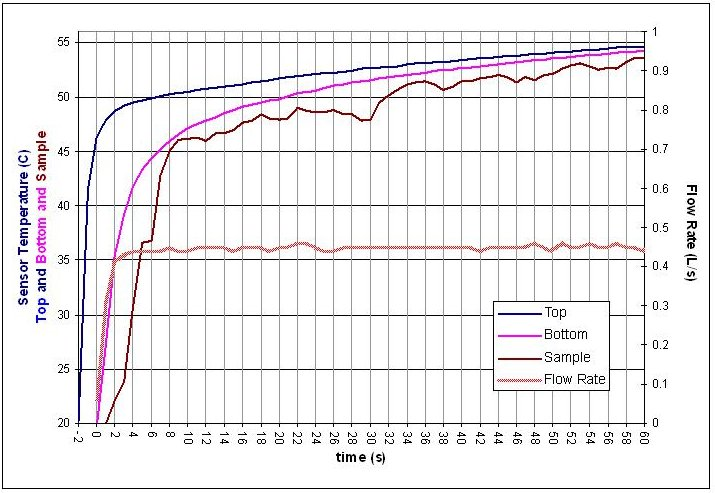
\includegraphics[scale=.65]{rawTemps.JPG}
\caption[Raw Temperature Plot]{\textbf{\emph{Raw Temperature Data from a Single Trial}} Temperature data sources depicted are top, bottom, and sample sensors with a flow rate plot on the right axis.\label{rawTemps}}
\end{center}
\end{figure}
\end{landscape}

\begin{table}[ht!]
\caption[Simulation Run-Time Statistics]{\textbf{Simulation Run Time Statistics}\label{runTime}}
\centering
\begin{tabular}{r l}
\hline
\hline
\\[-.5ex]
Data Time Resolution    & 1 second (all sensors)\\
\\
Reservoir Capacity	& $\lessapprox 40\;L$\\
\\
Reservoir Temperature 	& $43-51^{o}\;C$\\
\\
Fluid 			& Heated Tap Water\\
\\
Flow Rates		& 23 (Low), 41 (Med), 52 (High) $\frac{L}{s}$\\
\\
Flow Sensor		& $\frac{3}{4}''$ Digital Rotary Vane $\pm10\%$\\
\\
Flow Sensor Capacity	& 0.15 - 2.45 L/s\\
\\
Typical Flow Times (sec)& 190 (Low), 95 (Med), 65 (High)\\
\\
Sample Circuit Length	& 6.70 meters $\pm0.3\;m$\\
\\
Circuit Piping		& SCH 20 PVC $\frac{3}{4}''\varnothing$\\
\\
Vessel Dimensions	& 4'' x 27'' (10 x 69 cm)\\
\\
Vessel Volume		& 5.83 L\\
\\
Vessel Material		& SCH 40 PVC 4''$\varnothing$\\
\\
Typical Sample Mass	& 4.5-4.9 kg\\
\\
Pump Specification	& $\frac{1}{2}$ hp electric centrifugal @ $2000\;\frac{L}{hr}$\\
\\
\hline
\end{tabular}
\end{table} 

\subsubsection*{Apparatus Error and Calibration}
It was found that all samples were thermally exhausted within the amount of time 40 litres of water was flushed, regardless of rate, and this was the usual quantity circulated for a single trial. Background loss trials were performed demonstrating energy losses inside the vessel did not exceed the signal noise of the temperature sensors, and such this noise was not subtracted or otherwise considered in data analysis.

The flow sensor was calibrated using various known gravitationally driven flow rates. The circuit was plumbed to afford a continuous backpressure on the sensor to limit turbulent flow and air bubble contamination in the rotary vane cavity. Additionally, the effluent downspout was top vented so that the outflow would not siphon or draw additional flow through the sensor. Despite these provisions, the flow sensor was observed to ingest significant air and endure periodic turbulent flow, based on the driving flow rate. Further more, the rotary vane has a manufacturer tolerance of $\pm$10\%. While some of the turbulence and flow error has been absorbed into the interface calibration, the meter still demonstrated some error as a function of flow rate. For each trial, the reservoir was carfully filled to 40 litres (unless otherwise specified) and flow losses were neglected. A linear flow correction ratio was then computed for each data set.

\[flow\:correction\:ratio\;=\frac{measured\;cumulative\;flow}{measured\;reservoir\;volume}\]

In normalizing temperature differences and in an attempt to generate ideal data sets, the alternate warming circuit was used to achieve nominal differences between the top and reservoir temperatures at run time. Temperature differences between the top and reservoir sensors were never exactly $0^o\;C$ and varied exponentially as a function of time during the actual trial. This difference will partially be absorbed in the data analysis by only considering temperature differences across the vessel, but it will remain a known source of noise and curve distortion. 

The HOBO sensors were always calibrated and paired for use across the the vessel. However, no two sensors were measured to be exact, especially with respect to responsivity and accuracy. The sensors were not manufactured for fast responsivity and the aforementioned modifications increased the variability of each sensor, in exchange for dramatically faster responsivity. Variations in sensor readings were most notably manifested in offset equilibria, or a failure for the vessel temperature difference to reach $0^o\;C$, even when the aggregate was clearly thermally saturated. 

Because the temperature sensors were recording temperature continuously and were not triggered, the temperature data that was recorded across the sample vessel was unsynchronized with respect to the flow. The bottom temperature sensor was effectively reading the water temperature up to 6 seconds after the top sensor due to the vessel residency time of the flow. 

\[Vessel\:Residency\:Time\;=\;\frac{Vessel\:Length}{Flow\:Velocity}\]

\noindent Where the flow velocity is actually an involved empirical function of gravity, aggregate fineness, pump flow rate and aggregate packing ratio. This is discussed in the theory section. 

Sample, top and bottom temperature derivatives were plotted and time shifted such that the rise in temperature due to flow for each sensor was aligned in the time domain (refer to Data Analysis section). The time shift also offers an approximate determination for vessel residency time and vessel flow velocity. There is significant error in this detmination since both sensors cumulatively can produce an error of $\pm2$ seconds due to sampling syncopation and instrument timing variations. However, it does provide a useful baseline to compare flow differences between aggregates. 

Inflow was observed to be sufficiently turbulent such that there was no preferential flow into or about the sample. Additionally, all cobbles were noted to be equally well heated by touch upon emptying the vessel with no dry or cold ``spots''. Trials were run exclusively in ambient temperatures of $19-22^{o}\;C$. It has been hypothesized with some supporting data that the largest sources of error in the measurement of temperature was the sensors themselves and the variant reservoir temperatures.